\cotefile{157-5}

\scanpage{588}

\deleted{

\handwritten{\diagram{\begin{tikzcd}[ampersand replacement=\&,row sep=0.2em]
\unsure{\mathcal M|M}\mathbin{\overset{\mathrm{Loc}}{\boxtimes}}\unsure{\mathcal N|N}\\
\mathrel{\begin{tikzpicture}[baseline=-0.5ex]\node[rotate=90,inner sep=0pt]{$\simeq$};\end{tikzpicture}}\\
\underline{\mathrm{Hom}}^{!}_{\mathrm{Loc}}(\mathcal M^{\mathrm o},\mathcal N)
\end{tikzcd}}}

\handwritten{\[
\underbrace{\underline{\mathrm{Hom}}_{!\mathrm{Loc}}(\mathcal M,\deleted{\unsure{N}}\unsure{P|\mathcal P})}_{
\left\{\begin{gathered}
\inserted{\text{\unsure{des} }\underline{\mathrm{Hom}}\text{, et }\underline{\mathrm{Hom}}}\\
\text{\unsure{stables} par }\underset{\longrightarrow}{\lim}\\
\text{\unsure{localiseurs} }\inserted{\text{\unsure{Loc}}}\text{\unsure{-stables}}\\[-2pt]
\deleted{\unsure{P}}
\end{gathered}\right.}
\]}

\handwritten{$\boxed{\mathcal M,\mathcal N\quad\text{\unsure{Loc-paratopos|Loc-protopos}}}$

$P$ catégorie stable par p. $\underset{\longrightarrow}{\lim}$, \unsure{avec|un} localiseur \unsure{stable} par lesdites $\underset{\longrightarrow}{\lim}$.}

\handwritten{\[
\underline{\mathrm{Hom}}_{!\mathrm{Loc}}(\mathcal M\boxtimes\mathcal N,P)
\xrightarrow{\approx}\underline{\mathrm{Hom}}_{!\mathrm{Loc}}
(\mathcal M,\underline{\mathrm{Hom}}_{!\mathrm{Loc}}(\mathcal N,P))
\]}

\handwritten{\[
\begin{aligned}
f_i&\longrightarrow g_i\\
f=\underset{\longrightarrow}{\lim}\, f_i&\longrightarrow g=\underset{\longrightarrow}{\lim}\,g_i\\
f(\unsure{x|u})=\underset{\longrightarrow}{\lim}\,f_i(x)&\longrightarrow \begin{tikzpicture}[baseline=(term.base)]
\node[inner sep=0pt,outer sep=0pt] (term) {$\displaystyle g(x)=\underset{\longrightarrow}{\lim}\,g_i(x)$};
\draw[overlay,line width=.35pt]
 ([xshift=1em,yshift=5.4ex]term.north west)
 .. controls +(.05em,-1.8ex) and +(-.12em,.5ex) .. ([xshift=1.35em,yshift=.8ex]term.north west)
 .. controls +(.5em,1.1ex) and +(-1.5em,.4ex) .. ([xshift=-.5em,yshift=.8ex]term.north east)
 .. controls +(1.35em,-.25ex) and +(1.1em,.2ex) .. ([xshift=.16em,yshift=-.4ex]term.south east)
 .. controls +(-1.1em,-.6ex) and +(.8em,.15ex) .. ([xshift=1.2em,yshift=-.6ex]term.south west)
 .. controls +(-.6em,-.15ex) and +(.12em,1.2ex) .. ([xshift=.85em,yshift=-4.0ex]term.south west);
\end{tikzpicture}
\end{aligned}
\]}

\handwritten{\diagram{\begin{tikzcd}[ampersand replacement=\&,row sep=0.1em,column sep=small]
\unsure{f_g|f}(x) \& f(y)\arrow[l]\\
\begin{tikzpicture}[baseline=-0.5ex]\node[rotate=90,inner sep=0pt]{$\simeq$};\end{tikzpicture}
\&\begin{tikzpicture}[baseline=-0.5ex]\node[rotate=90,inner sep=0pt]{$\simeq$};\end{tikzpicture}\\
\underset{\longrightarrow}{\lim}\,f_i(x)\&\underset{\longleftrightarrow}{\lim}\,f_i(y)
\end{tikzcd}}}

\handwritten{Si $\mathcal M$ \deleted{\unsure{et}} et $\mathcal N$ \deleted{ont} des str. de Quillen spéciales, aussi $\mathcal M\mathbin{\overset{\mathrm{Loc}}{\boxtimes}}\mathcal N$ ? et $\underline{\mathrm{Hom}}_{!\mathrm{Loc}}(\mathcal M,N)$ ??}

\handwritten{\[
\mathcal M\mathbin{\overset{\mathrm{Loc}}{\boxtimes}}\deleted{\unsure{\mathcal C}}\widehat I
\mathrel{\overset{\mathrm{Loc}}{\underline{\approx}}}\mathcal M(I)
\qquad C_{\mathcal M}\boxtimes\mathrm{Fl}\,(\widehat I)
\]}

\handwritten{\[
\begin{gathered}
\begin{tikzpicture}[baseline=-0.5ex]\node[rotate=90,inner sep=0pt]{$\simeq$};\end{tikzpicture}\hfill\\[-2pt]
\underline{\mathrm{Hom}}^{!}(\widehat I^{\mathrm o},\mathcal M)
\approx(\underline{\mathrm{Hom}}_{!}(\widehat I,\mathcal M^{\mathrm o}))^{\mathrm o}
\approx(\underline{\mathrm{Hom}}(I,\mathcal M^{\unsure{\mathrm o}}))^{\mathrm o}
\approx\underline{\mathrm{Hom}}(I^{\mathrm o},\mathcal M)
\end{gathered}
\]}

\handwritten{\[
\begin{aligned}
\mathcal M\qquad W&=\mathrm{Is},\quad C\deleted{\unsure{of}}=\mathrm{Mon},\quad F\deleted{\unsure{ib}}=\mathrm{Ep}\ \mathrm{eff}.\\
\mathrm{TC}&=\mathrm{TF}=\mathrm{Is}
\end{aligned}
\]}

\handwritten{\diagram{\begin{tikzcd}[ampersand replacement=\&,row sep=small,column sep=small]
\&\deleted{C}\arrow[r,leftrightarrow] \& \deleted{\mathrm{TC}=\mathrm{Is}}\\
\deleted{\unsure{\mathrm T_y\mathrm F_{\mathrm{inj}}|\mathrm T\mathrm F_{\mathrm{inj}}}}\arrow[ur,dash] \& {}=C_* \arrow[r,leftrightarrow]\arrow[ur,dash,"{\unsure{-|\swarrow}}"'{pos=0.15}] \& F=\mathrm{Fl}
\end{tikzcd}}}

\handwritten{\diagram{\begin{tikzcd}[ampersand replacement=\&,row sep=small,column sep=small]
 C=\mathrm{Fl}^{\unsure{?|\times}}\arrow[r]\arrow[d,dash] \& \mathrm{TC}=\mathrm{Is}\arrow[d,dash]\\
 C_*=\mathrm{Is}=\mathrm{TF} \& F=\mathrm{Fl}\arrow[l]
\end{tikzcd}}}

}

% letterhead
% Printed upside down relative to the handwritten notes.
\noindent\begin{minipage}[t]{.48\linewidth}\raggedright\small
MINISTERE DE L'EDUCATION NATIONALE\\
\unsure{ACADEMIE} D'AIX-MARSEILLE\\
\hspace{2em}\rule{2cm}{0.3pt}\\
\unsure{Inspection} Académique\\
de Vaucluse\\
\hspace{2em}\rule{2cm}{0.3pt}\\
Tél. : 90 82 99 76\\
Référence : Secrétariat n°
\end{minipage}\hfill%
\begin{minipage}[t]{.48\linewidth}\raggedright\small
AVIGNON, le\\
L'Inspecteur d'académie,\\
directeur des services départementaux\\
de l'Education Nationale de Vaucluse,\\
à M
\end{minipage}

% archive sheet number: 587
\scanpage{589}

\handwritten{\fbox{p. 148-150} .}

% letterhead
\noindent\begin{minipage}[t]{.48\linewidth}\raggedright\small
MINISTERE DE L'EDUCATION NATIONALE\\
ACADEMIE D'AIX-MARSEILLE\\
\hspace{2em}\rule{2cm}{0.3pt}\\
Inspection Académique\\
de Vaucluse\\
\hspace{2em}\rule{2cm}{0.3pt}\\
Tél. : 90 82 99 76\\
Référence : Secrétariat n°
\end{minipage}\hfill%
\begin{minipage}[t]{.48\linewidth}\raggedright\small
AVIGNON, le\\
L'Inspecteur d'académie,\\
directeur des services départementaux\\
de l'Education Nationale de Vaucluse,\\
à M
\end{minipage}

\handwritten{\uline{\unsure{Op.} $\cdot\ x\boxtimes y$}}

\handwritten{\textcircled{1}\quad $\underline{\mathrm{Hom}}_{!}(\unsure{\mathcal M|M},\unsure{\mathcal N|N})\qquad\mathcal M\boxtimes\mathcal N$\quad \unsure{associés|associées} par}

% slanted
\handwritten{\margin{propriété universelle}}

\handwritten{\[
\left|\begin{aligned}
\underline{\mathrm{Hom}}(\mathcal M\boxtimes\mathcal N,P)&\mathrel{\underline{\approx}}\unsure{\underline{\mathrm{Hom}}|\text{\uuline{Hom}}}(\mathcal M,\underline{\mathrm{Hom}}_{!}(\mathcal N,P))\\
&\mathrel{\underline{\approx}}\underline{\mathrm{Hom}}(\mathcal N,\underline{\mathrm{Hom}}_{!}(\mathcal M,P))\\
\deleted{\unsure{H}}&\mathrel{\underline{\approx}}\mathrm{Hom}_{!!}(\mathcal M,\mathcal N;P)
\end{aligned}\right\}\ \text{\unsure{vrai} iso}
\]}

\handwritten{\[
\mathcal M\boxtimes\mathcal N\quad\left|\begin{aligned}
&\text{comm. à isom. près}\\
&\text{assoc. à équiv. \unsure{près|pres}}\\
&\mathrm{Ens}\ \text{est l'objet unité bilatère}
\end{aligned}\right.
\]}

\handwritten{\[
\text{\textcircled{2}}\quad\mathcal M_{\unsure{\pi|\kappa}}\boxtimes\mathcal N_\pi
\mathrel{\unsure{-|\longrightarrow}}(\mathcal M\boxtimes\mathcal N)_\pi
\overset{\mathrm{\unsure{déf|def}}}{=}\mathcal M_\pi\boxtimes\mathcal N_\pi
\]}

\handwritten{Question : si $\pi$ est utile pour $\mathcal M$ et pour $\mathcal N$, l'est-il pour $\mathcal M\boxtimes\mathcal N$ ? Oui !}

\handwritten{plus précisément}

\handwritten{\[
S\mathbin{\overset{\pi}{\boxtimes}}T\simeq
\bigl(\mathrm{Ind}_\pi(S)\boxtimes\mathrm{Ind}_\pi(T)\bigr)_\pi
\]}

\handwritten{\unsure{donc|de} \unsure{sorte} \unsure{que}}

\handwritten{\[
\mathrm{Ind}_\pi(S\mathbin{\overset{\pi}{\boxtimes}}T)
\mathrel{\overset{\text{\textcircled{?}}}{\underline{\approx}}}
\mathrm{Ind}_\pi(S)\boxtimes\mathrm{Ind}_\pi\unsure{(T)}
\]}

\handwritten{\deleted{$\unsure{\pi}\quad\underline{\mathrm{Hom}}^{!!\pi,}(S^{\mathrm o},T^{\mathrm o},\mathrm{Ens})\mathrel{\overset{?}{\underset{\longleftarrow}{\approx}}}\mathrm{Ind}_\pi($}}

\handwritten{\textcircled{3}\quad \unsure{Espèces|Espèce} de structures algébriques dans $\unsure{\mathcal U|U}$. \unsure{Correspondant|Correspondent} aux $\mathcal U$-\unsure{paratopos|protopos}. \unsure{Interpréter} $\mathcal M\boxtimes\mathcal N$. Y-a-t-il \unsure{une} pour $\underline{\mathrm{Hom}}_!(\mathcal M,\mathcal N)$ ? J'en doute\ldots}

% archive sheet number: 588
\scanpage{590}

\textcircled{4}\quad Cas des $\mathrm{Ind}(C)$ i.e. des \inserted{$\unsure{\mathcal U|U}$-}\unsure{paratopos|protopos} \inserted{($C$ stable par $\underset{\longrightarrow}{\lim}$ finies)} à \unsure{eng.|cog.|cond.} de prés. finie. On a

\[
\mathrm{Ind}(S)\boxtimes\mathrm{Ind}(T)\simeq\mathrm{Ind}(S\mathbin{\overset{1}{\boxtimes}}T)
\]

où

\[
\begin{aligned}
S\mathbin{\overset{\deleted{\unsure{1}}f}{\boxtimes}}T
&\mathrel{\overset{\mathrm{\unsure{déf|def}}}{=}}\bigl(\mathrm{Ind}(S)\boxtimes\mathrm{Ind}(T)\bigr)_{\mathrm{PF}}\\
&\simeq\bigl(\mathrm{Hom}^{!!f.}(S^{\mathrm o},T^{\mathrm o};\mathrm{Ens})\bigr)_{\mathrm{PF}}\\
&\hspace{7em}\cap\\
&\hspace{5em}(S\times T)^{\wedge}_{\mathrm{PF}}
\end{aligned}
\]

\uline{NB}\quad Les opérations $\unsure{\mathcal M|M}\mathbin{\overset{\unsure{\pi|\kappa}}{\boxtimes}}\unsure{\mathcal N|N}$ pour $\pi$ \unsure{cardin.|cardinal} \unsure{transfini|infini}, ou $\pi=f$, \unsure{finies|fini}, \deleted{\unsure{ou}} sur les catégories qui sont stables par $\underset{\longrightarrow}{\lim}$ de \unsure{cardinal} $\leq\pi$ (resp. par $\underset{\longrightarrow}{\lim}$ finies), est comm. à isom près, et associatif et unitaire à équiv. près. L'objet unité est $\mathrm{Ens}_\pi$ resp. $\mathrm{Ens}_f$.

\figure{\begin{tikzpicture}
\node[inner sep=0pt] (symbol) {$\unsure{\mathbb P|P}\mathbin{\underset H\wedge}\unsure{\mathbb Q|Q}$};
\node[inner sep=0pt,anchor=west,text width=.65\linewidth,align=left] (words) at ([xshift=1.8em]symbol.east)
 {si $P$ et $Q$ sont des $H$-gerbes (sur un topos) $H$ faisceau abélien. C'est une opération associative, comm., \unsure{unitaire} à \unsure{équivalence} près\ldots.};
\draw[line width=.4pt] ([xshift=-1em]symbol.west)
 .. controls +(-.15em,3ex) and +(-2em,-.3ex) .. ([yshift=.45ex]words.north west)
 .. controls +(2.2em,.3ex) and +(-.8em,.55ex) .. ([xshift=-.75em,yshift=.95ex]words.north east)
 .. controls +(1em,-.1ex) and +(.08em,1ex) .. ([xshift=.25em,yshift=.8ex]words.east);
\draw[line width=.4pt] ([xshift=-1em,yshift=-.2ex]symbol.west)
 .. controls +(.15em,-2.7ex) and +(-1.8em,.25ex) .. ([yshift=-.6ex]words.south west);
\draw[line width=.4pt] ([xshift=.3em,yshift=-.7ex]words.south)
 .. controls +(1.4em,.2ex) and +(-.7em,-.55ex) .. ([xshift=.15em,yshift=.15ex]words.south east);
\draw[line width=.35pt] ([xshift=-1.5em,yshift=2.1ex]words.north west) -- ([xshift=3.2em,yshift=2.6ex]words.north west);
\end{tikzpicture}}

% archive sheet number: 589
\scanpage{591}

\noindent\hfill Appendice \unsure{à|:} $\overline{\underline{\mathrm{XVIII}}}$

% archive sheet number: 590
\scanpage{592}

\mspage{\uline{1}}

% slanted
\margin{\uline{Appendice} \unsure{:|à} \uline{XVIII}}

Ultraproduits de corps, et catégories accessibles.

Soit $(k_{\unsure{\xi|\zeta}})_{\xi\in E}$ une famille de corps, \unsure{indexé|indexée} par un ens. $E$, \deleted{et} [Soit $\Phi$ un filtre non trivial dans $E$, i.e. une partie $\Phi\subset\unsure{\mathcal P|\mathfrak P}(E)$ telle que \deleted{\unsure{a)} $\Phi$} a) $\varnothing\notin\Phi$ i.e. $A\in\Phi\Longrightarrow A\ne\varnothing$ b) $A,B\in\Phi\Longrightarrow A\cap B\in\Phi$, et \unsure{c)} si $A\in\Phi$, $A\subset B$ alors $B\in\Phi$, \inserted{d) $\Phi\ne\varnothing$ $(\Longleftrightarrow E\in\Phi)$} \deleted{Cela revient} à dire que

$\Phi$ est une partie \unsure{fermée|finie} de l'ens. ordonné $\mathcal P(E)$, \uline{\unsure{filtrante} à gauche}, et ne \unsure{contient} pas le plus petit \unsure{élémt|él'mt|élément} de $\mathcal P(E)$, i.e. non égal à $\mathcal P(E)$ \deleted{\unsure{tout}} entier.)] Pour tte partie $J$ de $E$, posons

\[
k_J=\prod_{\xi\in J}k_\xi\ ,
\]

\deleted{\unsure{on|et}} \deleted{\unsure{sait}} \unsure{c|ça} \unsure{donne} \deleted{\unsure{un}} un système projectif \deleted{\unsure{cofiltrant}}

\[
(k_J)_{J\in\mathcal P(E)},\qquad
\left|\begin{aligned}&\text{i.e. }J\subset J'\ \text{donne}\\[-2pt]
&k_{J'}\mathrel{\unsure{-|\to}} k_J
\end{aligned}\right.
\]

et \deleted{\unsure{la}} le système

\[
(k_J)_{J\in\Phi}
\]

est un système inductif d'anneaux, indexé par l'ens ordonné filtrant $\Phi^{\mathrm o}$\unsure{:|;} Posons

\[
k_\Phi=\underset{\substack{\longrightarrow\\J\in\Phi}}{\lim}k_J\ .
\]

Si $\Psi$ est un filtre plus fin que $\Phi$, \unsure{i.e.}

% archive sheet number: 591
\scanpage{593}

\mspage{2}

tel que $\Psi\supset\Phi$, on \unsure{trouve} un hom. can.

\[
k_\Phi\mathrel{\unsure{\longrightarrow|-}} k_\Psi\ ,
\]

donc si $\unsure{\mathscr F|\mathcal F}(E)=\mathscr F$ est l'ens des \deleted{\unsure{en}} filtres sur $E$, ordonnés par inclusion, on trouve un système inductif

\[
\Phi\mathrel{\unsure{\mapstochar\relbar|\longmapsto}} k_\Phi:\quad\mathscr F\longrightarrow\mathrm{Ann}
\]

On n'a pas utilisé encore que les $k_{\unsure{\xi|\zeta}}$ sont des corps, en fait il suffisait que ce soient des objets d'une catégorie $\unsure{\mathcal A|A}$ stable par \inserted{petits produits} \inserted{et par} petites $\underset{\longrightarrow}{\lim}$ filtrantes. Prenons maintenant $\mathcal A=\mathrm{Ann}$ (catégorie des anneaux unitaires, non néc. commutatifs), et supposons que les $k_\xi$ soient des corps.

\uline{Proposition 1} \inserted{Supposons que les $k_\xi$ $(\xi\in E)$ soient des \uline{corps}.$^{*}$} Pour que $k_\Phi$ soit un corps, il f et s. que $\Phi$ soit un ultrafiltre, i.e. que pour toute \deleted{partie $A$ de \deleted{\unsure{$\mathcal P(E)$}} $E$, on ait $A\in\Phi$ ou $\complement_E A$} \inserted{décomposition $E=A\amalg B$, on ait} $A\in\Phi$ ou $B\in\Phi$. (NB. Si $A\in\Phi$, on a $B\notin\Phi$, puisque sinon on aurait $A\cap B\in\Phi$ donc $\varnothing\in\Phi$, absurde.)

% slanted
\margin{$^{*}$NB. Cette condition est \unsure{nécessaire}, si on veut que $k_\Phi$ soit un corps pour \unsure{tout} ultrafiltre \unsure{p.|pr.} $\Phi$.}

Nécessité : Soit, pour \unsure{tte|tt|toute} partie $A$ de $E$,

\[
\unsure{f_A|\varphi_A}\in k_E\quad\text{défini par}\quad f_A(\xi)=
\begin{cases}
1_{k_\xi}&\text{si }\xi\in A\\
0_{k_\xi}&\text{si }\xi\in E\setminus A\ .
\end{cases}
\]

% archive sheet number: 592
\scanpage{594}

\mspage{3}

\unsure{-} Soit

\[
\unsure{f_{A,\Phi}|\varphi_{A,\Phi}}\in k_\Phi
\]

l'image de $f_A$ par \inserted{l'hom. can.} $k_E\longrightarrow k_\Phi$. Si $E=A\amalg B$ on aura

\[
f_A+f_B=1,\quad f_A f_B=0
\]

d'où

\[
f_{A,\Phi}+f_{B,\Phi}=1,\quad f_{A,\Phi}f_{B,\Phi}=0\ .
\]

Si $k_\Phi$ est un corps, cela implique que \deleted{$\unsure{f_A J}$} on a $f_{A,\Phi}=0$ ou $f_{B,\Phi}=0$. Mais si p.ex. $f_{A,\Phi}=0$, on voit que cel\unsure{a} signifie que il existe un $J\in\Phi$ tel que $f_A\mid J=0$, ce qui signifie aussi que $J\subset B$. De $=$, si $f_{B,\Phi}=0$, on aura $J\subset A$. Donc $\Phi$ est un ultrafiltre.

Inversement, supposons que $\Phi$ soit un ultrafiltre. \deleted{Alors} Prouvons que $k_\Phi$ est un corps, i.e. que pour $f\in k_\Phi$, $f\ne0\Rightarrow f$ inversible.

\deleted{Mais $f=0$ signifie qu'il} Notons que $f$ provient d'un $\unsure{g}$ \unsure{élmt|él'mt} d'un $k_{\deleted{\unsure{B|D}}J}$ $(J\in\Phi)$, donc est l'image canonique d'un $g\in k_E$. Dire que $f=0$ signifie que $\exists\ J\in\Phi$ tel que $g\mid J=0$. L'inverse \inserted{$f\ne0$} signifie donc que pour tt $J\in\Phi$, on a $g\mid J\ne0$.

% archive sheet number: 593
\scanpage{595}

\mspage{4}

Soit alors $A$ l'ens des $\unsure{\xi|\zeta}\in E$ tels que $g(\xi)\ne0$, $B=E\setminus A$ l'ens des $\xi\in E$ tels que $g(\xi)\unsure{\ne|=}0$. \inserted{On a donc $B\notin\Phi$ \deleted{\unsure{parce que|puisque}} puisque $f\ne0$, et} comme $\Phi$ est un ultrafiltre, on a donc $A\in\Phi$.

Mais soit $g'\inserted{\in k_E}$ défini par $g'(\xi)=f(\xi)^{-1}$ si $\xi\in A$, \inserted{$g'(\xi)=1$ si $\xi\in B$,} et soit $f'$ l'image de $g'$ dans $k_\Phi$. On voit alors qu'on a

\[
ff'=f'f=1\ ,
\]

ce qui montre bien que $k_\Phi$ est un corps.

Supposons maintenant que tous les $k_\xi$ $(\xi\in E)$ soient égaux à un $=$ corps $k$. Alors les $k_J$ \unsure{forment} un système projectif de $k$-algèbres, les $k_\Phi$ un syst. inductif de $k$-algèbres. Si $k$ est commutatif, il en est de $=$ des $k_J$, $k_\Phi$, et en particulier \unsure{pour} $\Phi$ un ultrafiltre, $k_\Phi$ est une \uline{extension} du corps $k$.

Revenons au cas général, \inserted{mais les $k_\xi$ comm.} \deleted{je dis que} \inserted{Soit} \deleted{\uline{Proposition}} $\unsure{\mathscr F|\mathcal F}_0\subset\mathscr F$ l'ens des ultrafiltres sur $E$,

Notons que pour $\unsure{\forall|\mathrm{tt}}\Phi\in\mathscr F$, $k_E\mathrel{\unsure{-|\to}}k_\Phi$ est surjectif. Donc si $\Phi\in\mathscr F_{\unsure{0}}$, $k_\Phi$ s'identifie à un corps quotient de l'\unsure{anneau} $k_E$.

% archive sheet number: 594
\scanpage{596}

\mspage{5}

\deleted{Soit $\mathrm{Max}(k_E)$ l'ens \deleted{des} le spectre maximal de $k_E$,}

Pour $\unsure{\forall|\mathrm{tt}}$ anneau $A$, soit $\mathrm{Max}(A)$ \unsure{son|le} spectre maximal, i.e. l'ens des idéaux \unsure{maxima|maximaux} de $A$. On \unsure{trouve} donc une application canonique

\[
\left|\begin{aligned}
\unsure{\mathscr F|\mathcal F}_0&\longrightarrow\mathrm{Max}(k_E)\\
\Phi&\longmapsto\mathrm{Ker}(k_E\longrightarrow k_\Phi)\overset{\mathrm{\unsure{déf|def}}}{=}\unsure{\mathfrak m|m}_\Phi
\end{aligned}\right.\tag*{\makebox[0pt][r]{\makebox[\displaywidth][l]{\unsure{(a)|(A)}}}}
\]

\uline{Proposition 2}\qquad L'application précédente est \uline{bijective}.

\unsure{Prouvons} d'abord qu'elle est injective, cela \deleted{provient de} résulte aussitôt du

% slanted
\margin{Cf \unsure{ci-après} pour \unsure{le} cor. 3 c), pour $\Phi$ filtre quelconque}

\uline{Corollaire 1}\qquad Soit, pour $\Phi\in\mathscr F_0$,

\[
\unsure{\chi|X}_\Phi:k_E\mathrel{\unsure{-|\longrightarrow}}k_\Phi
\]

l'application canonique. Alors pour $A\in\unsure{\mathcal P|\mathfrak P}(E)$, on a

% slanted
\margin{\uline{NB} Pour $\Phi\in\mathscr F$ quelconque, $\mathfrak m_\Phi\overset{\mathrm{def}}{=}\mathrm{Ker}(\chi_\Phi:k_E\mathrel{\unsure{-|\to}} k_\Phi)$ détermine $\Phi$, puisque $A\in\Phi\Longleftrightarrow\chi_\Phi(\unsure{f_A|\varphi_A})=1$ (mais il faut \unsure{supposer} les $k_{\unsure{\xi|\zeta}}\ne0$, i.e. $0_\xi\ne1_\xi$ \unsure{\ldots})}

% slanted
\margin{\deleted{$k_\xi$} \unsure{remonter|remonté|anneaux} \uline{\unsure{avant|unit}} \unsure{corps}}

\[
\begin{aligned}
 A\notin\Phi&\Longleftrightarrow\chi_\Phi(f_A)\unsure{=|\ne}0\quad\text{i.e. } f_A\in\mathfrak m_\Phi\\
 \text{(i.e. }\ A\in\Phi&\Longleftrightarrow\chi_\Phi(f_A)\ne0\quad\text{i.e. } f_A\notin\mathfrak m_\Phi).
\end{aligned}
\]

% slanted
\margin{\uline{NB} \unsure{bien sûr} $(\chi_\Phi(f_A)\ne0)\Longleftrightarrow(\chi_\Phi(f_A)\unsure{=1|\ne1})$}

En effet, $\chi_\Phi(f_A)=0$ signifie qu'il existe $B\in\Phi$ tel que $f_A\mid B=0$, i.e. tel que $B\subset E\setminus A$; mais \deleted{\unsure{cela}} \deleted{$E\setminus A\in\Phi$, et} équivaut à $E\setminus A\in\Phi$, donc \unsure{à|:} $A\notin\Phi$ puisque $\Phi$ est un ultrafiltre, qed.

% archive sheet number: 595
\scanpage{597}

\mspage{6}

\unsure{.} Reste à prouver que l'application (\unsure{a|A}) est \unsure{surjectif|surjective}. Soit donc $\unsure{\mathfrak m|m}$ un idéal maximal de $k_E$, et soit

\[
\Phi\overset{\mathrm{def}}{=}\{A\in\unsure{\mathcal P|\mathfrak P}(E)\mid \deleted{\unsure{f_A\notin\mathfrak m}}\ \text{\unsure{i.e.|t.q.} }\unsure{\chi|X}(\unsure{f_A|\varphi_A})\deleted{\unsure{\ne0}}\unsure{=1|\ne1}\},
\]

où $\chi:k_E\mathrel{\unsure{-|\longrightarrow}} k_E/\mathfrak m\inserted{=k(\mathfrak m)}$ est l'application canonique.

Je dis que $\Phi$ est un ultrafiltre. En effet, a) $\varnothing\notin\Phi$ car $f_\varnothing=0$ \inserted{d'où $\chi(f_\varnothing)=0\ne\deleted{\unsure{0}}1$ dans $k_\Phi$}, b) si $A,B\in\Phi$, on a \deleted{\unsure{$f$}} $A\cap B\in\Phi$, car $f_{A\cap B}=f_A\cdot f_B$ d'où $\chi(f_{A\cap B})=\chi(f_A)\chi(f_B)\deleted{\unsure{\ne}}\unsure{=1|\ne1}$,

c) Si $A\subset B$ et $A\in\Phi$, alors $B\in\Phi$, \deleted{en effet i.e. $B\notin\Phi\Rightarrow A\notin\Phi$} \deleted{on a $f_A f_B=\unsure{f_A}$,} \deleted{ou encore $\chi(f_B)=0\Rightarrow\chi(f_A)=0$.} En effet, on a $f_A=f_A f_B$, d'où $\chi(f_A)=\chi(f_A)\chi(f_B)$, \inserted{et comme $\chi(f_A)=1$, on trouve $\chi(f_B)=1$}

\deleted{\unsure{D'où} la \unsure{condition|conclusion}} d) On a $E\in\Phi$, i.e. $\chi(f_E)\deleted{\unsure{\ne}}=1$, or $f_E=1$ donc $\chi(f_E)=1$. \deleted{\unsure{Enfin},}

Ainsi, $\Phi$ est un filtre, \deleted{\unsure{puisqu'on a jusqu'ici} \unsure{utilisé} $\ne0$, et} \inserted{on n'a utilisé que le fait que $A/\mathfrak m$ est \deleted{\illegible{2}} un anneau $\ne0$ (pour \unsure{conclure} \unsure{que} $\varnothing\notin\Phi$).} \deleted{on \unsure{voit ici}} \deleted{\unsure{il faut|pour} un corps} \deleted{\unsure{Utilisons} Mais} \inserted{$A/\mathfrak m$ est intègre,} Prouvons que \deleted{si \unsure{$\mathfrak m$ est maximal},} \deleted{donc} $\Phi$ est un \uline{ultrafiltre}, ie. \unsure{a)} si $A\notin\Phi$, alors $B\overset{\mathrm{def}}{=}E\setminus A\in\Phi$.

En effet on a \deleted{\unsure{b)}} $f_A+f_B=1$, \deleted{$f_Af_B=0$, d'où $\chi(f_A)+\chi(f_B)=1$} \deleted{$\chi(f_A)\chi(f_B)=0$,} \inserted{$f_A f_B=0$, d'où \textcircled{a} $\chi(f_A)+\chi(f_B)=1$, et \textcircled{b} $\chi(f_A)\chi(f_B)=0$;} \deleted{Comme $\chi(f_A)=\unsure{0|2}$, c'est $\chi(f_B)=1$} $\chi(f_A)\ne1$, on conclut de \textcircled{a} $\chi(f_B)\ne0$, d'où de \textcircled{b} $\chi(f_A)=0$, d'où de \textcircled{a} $\chi(f_B)=1$. D'où $B\in\Phi$.

% archive sheet number: 596
\scanpage{598}

\mspage{7}

Prouvons enfin que $\unsure{\mathfrak m|m}=\mathfrak m_\Phi$. Comme $\mathfrak m_\Phi$ est un idéal maximal, il suffit de prouver

\[
\mathfrak m_\Phi\subset\mathfrak m\ .
\]

Or si $A\in\unsure{\mathcal P|\mathfrak P}(E)$ est telle que $A\notin\Phi$, \deleted{\unsure{ou $f$}} \unsure{i.e.|c.à.d.} $\unsure{f_A|\varphi_A}\in\mathfrak m_\Phi$ \deleted{\unsure{$=$}} (cor. 1), on a aussi $f_A\in\mathfrak m$. Donc il suffit de prouver le

\uline{Lemme}. Soit $\Phi\in\unsure{\mathscr F|\mathcal F}_0$. Alors $\mathfrak m_\Phi$ est \deleted{\unsure{le}} l'idéal engendré par les $f_A$ pour $A\in\mathcal P(E)\setminus\Phi$\inserted{, et \deleted{\unsure{même}} plus précisément, ces $f_A$ sont dans $\mathfrak m_\Phi$, et tt $f\in\mathfrak m_\Phi$ est de la forme $ff_A$, avec $A$ \unsure{au|et} \unsure{comme} \unsure{ci-dessus}}.

\deleted{Soit} En effet, $f\in\mathfrak m_\Phi$ signifie qu'il existe $B\in\Phi$ tel que $f\mid B=0$. Mais cela signifie aussi que $f=ff_A$, où $A=E\setminus A$, d'où $A\notin\Phi$. \deleted{Cela \unsure{montre} que $f$}

\inserted{Cela prouve la proposition 2, et en $=$ temps :}

\uline{Corollaire 2}. Tout anneau quotient intègre de $k_E=\prod_{\unsure{\xi|\zeta}\in E}k_\xi$ est un corps.

\deleted{\uline{\unsure{Corollaire 2}}} Notons \unsure{maintnt|maintenant} que si $\Phi\in\mathscr F$ est un filtre quelconque \deleted{de} $E$, alors $k_\Phi$ est un anneau quotient de $k_E$, donc

\diagram{\begin{tikzcd}[ampersand replacement=\&,row sep=0.1em,column sep=small]
\text{\unsure{(a)|(A)}}\quad\&\mathrm{Max}(k_\Phi)\arrow[r,hook]\&\mathrm{Max}(k_E)\ .\\
\&\&\begin{tikzpicture}[baseline=-0.5ex]\node[rotate=90,inner sep=0pt]{$\simeq$};\end{tikzpicture}\\
\&\&\mathscr F_0
\end{tikzcd}}

% slanted
\margin{\unsure{Notons} pour tt système d'anneaux $(k_\xi)_{\xi\in E}$ \uline{\unsure{non nuls|tous unit.}}, et $\Phi,\Psi\in\mathscr F$ \deleted{\unsure{sif}} ($\Psi$ plus fin que $\Phi$ \unsure{(i.e. $\Phi\subset\Psi$)}) sss $\mathfrak m_\Phi\subset\mathfrak m_\Psi$ (\unsure{suffira|suffit|supposer} le \unsure{premier} \unsure{filtre|ultrafiltre}, \unsure{soit} \unsure{surj.|sans} \illegible{1}).}

Ceci \unsure{posé|précisé}, on trouve

\uline{Corollaire 3} : \deleted{\unsure{Les}} L'inclusion précédente identifie $\mathrm{Max}(k_\Phi)$ à l'ens des ultrafiltres $\Psi$ sur $E$ qui sont \uline{plus fins} que $\Phi$.

En effet, si $\Psi$ est un tel ultrafiltre, on

% archive sheet number: 597
\scanpage{599}

\mspage{8}

a le diagramme commutatif

\diagram{\begin{tikzcd}[ampersand replacement=\&,column sep=small]
\text{\unsure{(a)|(u)}}\quad\&k_E\arrow[r,dash,"\unsure{\chi|X}_\Phi","{\unsure{-|\to}}"{pos=1,anchor=center}]\arrow[rr,dash,bend right=24,"\chi_\Psi"',"{{\unsure{-|\to}}}"{pos=1,anchor=center}]\&k_\Phi\arrow[r]\&k_\Psi\ ,
\end{tikzcd}}

ce qui montre que $\Psi$ est dans l'image de \unsure{(a)|(u)}. Inversement, supposons que $\Psi\in\unsure{\mathscr F|\mathcal F}_0$ provienne de $\mathrm{Max}(k_\Phi)$, i.e. qu'\deleted{il existe $k_\Phi\to k_\Psi$}\inserted{l'on ait \deleted{\unsure{un}}} \deleted{\unsure{$f$}} $\unsure{\mathfrak m|m}_\Phi\subset\mathfrak m_\Psi$ \deleted{\unsure{(}} (\unsure{où|i.e.} $\mathfrak m_\Phi$ est le noyau de $\chi_\Phi$), ou encore qu'on ait une factorisation (a) de $\chi_\Psi$.

Prouvons que $\Psi$ est plus fin que $\Phi$, i.e. que $\Psi\supset\Phi$. Soit donc $A\in\Phi$, prouvons que l'on a $A\in\Psi$. \deleted{Cela va résulter du} \inserted{Mais $A\in\Phi$ \unsure{implique|signifie}} \deleted{Si on avait $A\notin\Psi$, on} fait que \deleted{\unsure{$f$}} $\chi_\Phi(\unsure{f_A|\varphi_A})=1$ \deleted{est \uline{inversible} dans $k_\Phi$,} \deleted{en conclurait que $f_A\in\mathfrak m_\Psi$} donc son image dans $k_\Psi$ est \deleted{\unsure{une unité|non nulle},} égale à 1, donc on a $A\in\Psi$ par le cor. 1. \deleted{\unsure{précédent}, Je \unsure{ferai}} \deleted{\unsure{donc} j'\unsure{utiliserai} ledit corollaire \unsure{ainsi} :}

\deleted{

% slanted
\margin{\unsure{remonté} à la place du cor. 1}

\uline{Corollaire 3} (de prop. 2) Soit $\Phi$ un filtre sur $\unsure{k|E}$. \deleted{Alors \unsure{$\Phi$} $A\in\Phi$} et $A\in\unsure{\mathcal P|\mathfrak P}(E)$. Alors

\[
A\in\Phi\Longleftrightarrow\chi_\Phi(f_A)\ \text{est inversible dans }k_\Phi
\]

(\unsure{donc|avec} $\Phi$ est \unsure{connu}, quand on \unsure{connait|connaît} l'anneau quotient $\chi_\Phi$ de $k_E$).
}

% archive sheet number: 598
\scanpage{600}

\mspage{9}

Supposons à présent que tous les $k_{\unsure{\xi|\zeta}}$ soient égaux au même \deleted{corps commutatif $k$}\inserted{anneau $\boxed{k\ne0}$}. \deleted{Donc les} \deleted{des lors $\Phi$ est un ultrafiltre, $k_\Phi$ est une extension \unsure{de}} \inserted{$k\mathrel{\unsure{-|\to}}k_J\mathrel{-}k_\Phi$} les $k_J$, $k_\Phi$ sont des \deleted{$k$-algèbres,}\inserted{``anneaux sur $k$''}, d'ailleurs $k\mathrel{\unsure{-|\to}}k_{\unsure{\Phi|J}}$ \inserted{(si $J\ne\varnothing$) et $k\mathrel{-}k_\Phi$} est injectif. On se pose la question quand \inserted{$k\mathrel{-}k_\Phi$} c'est \uline{bijectif}, i.e surjectif. Comme $k_\Phi\simeq k_E/\unsure{\mathfrak m|m}_\Phi$, cela signifie donc que $k_E=k+\mathfrak m_\Phi$, i.e que \deleted{de tte} $f\in k_E$ s'écrit

\[
 f=c+g\qquad\left|\begin{aligned}
 &c\in k\quad\text{i.e. }\ c(\xi)=\underset{\substack{\begin{tikzpicture}[baseline=-0.4ex]\node[inner sep=0pt,rotate=90]{$\in$};\end{tikzpicture}\\ k}}{c_0}\quad\forall\xi\in E\\
 &g\in\mathfrak m_\Phi\quad\text{i.e. }\ \exists A\in\Phi\ \text{avec}\\
 &\hspace{9em} g\mid A=0\ .
 \end{aligned}\right.
\]

Mais pour $f\inserted{\in k_E},\ c\in k$ \inserted{et $A\in\Phi$} fixés, l'existence de $g\in \deleted{\unsure{k_\Phi}} k_E$ \deleted{et $A\in\Phi$ comme dessus,} \deleted{tels qu'on ait $f=c+g$, équivaut à l'existence} \inserted{tels que $g\mid A=0$ et $f=c+g$ équivaut} \deleted{de $A\in\Phi$} à \deleted{\unsure{i.e.} $A\subset$} $f\mid A=c_A$, \unsure{(}fonction \unsure{constte|constante} \unsure{sur|de} $A$, de valeur $c$) \inserted{i.e. $A\subset f^{-1}(\{c\})$. Pour $f,c$ fixés, l'existence} \deleted{\unsure{Donc}} de $A\in\Phi$ \deleted{qui \unsure{ait}} \unsure{satisfaisant} ces relations équivaut à $f^{-1}(\{c\})\in\Phi$.

% slanted
\margin{Et pour $f$ fixé, l'exist\textsuperscript{ce} de $c$ équivaut à celle d'une fibre $E_c$ de $f:E\mathrel{\unsure{-|\to}}k$, qui soit dans $\Phi$. D'où}

\uline{Proposition 3} Soit \deleted{$H=\mathrm{Card}\,k$, et} $\Phi\in\unsure{\mathscr F|\mathcal F}$. Pour que $k\mathrel{-}k_\Phi$ soit surjectif, il \unsure{f} et il suffit que pour \deleted{toute constante, \unsure{les}} famille de parties \inserted{\uline{mutuellement disjointes}} $(E_\xi)_{\xi\in k}$ de $E$ indexée par $k$, \deleted{telle qu'on ait} \inserted{de réunion} $E$, \deleted{\unsure{$=\bigcup E_\xi$}} il existe un $\xi\in k$ tel que $E_\xi\in\Phi$. A fortiori, il \uline{faut} que $\Phi$ soit un ultrafiltre (puisque $\unsure{\mathrm{Card}|\mathrm{card}}\,k\geq2$ par hypothèse).

% archive sheet number: 599
\scanpage{601}

\mspage{10}

En effet, la donnée d'une telle famille $(E_{\unsure{\xi|\zeta}})_{\xi\in k}$ équivaut à la donnée d'une application $E\unsure{-|\to}k$, i.e. d'un \unsure{élmt} de $\unsure{f_E|k_E}$. \deleted{\unsure{Et}}

\deleted{\unsure{S|B}} \uline{Scholie} La propriété qu'on vient d'expliciter, pour un filtre $\Phi$\inserted{, sur $E$}, ne dépend \deleted{que} de $k$ que par l'intermédiaire de $\unsure{\pi|\kappa}=\operatorname{card}k$. On peut aussi l'énoncer en disant que pour tte \uline{partition} $(E_i)_{i\in I}$ de $E$ en \inserted{un ens. $I$ de} parties tel que $\operatorname{card}I\leq\pi$, il existe un (et un seul) des $E_i$ qui soit dans $\Phi$. On dit alors que $\unsure{Q|\Phi}$ est un $\pi$-ultrafiltre.

Si $\pi\geq 2$ est fini, cette propriété équivaut à dire que $\Phi$ est un ultrafiltre. \deleted{Si $\pi$ est infini, il n'est pas clair qu'il \unsure{existe|a}} \inserted{Par ailleurs, quel que soit $\pi$, les} ultrafiltres $\Phi$ \uline{triviaux} \unsure{(}(i.e. tels qu'il existe $\xi\in E$ avec $\{\xi\}\in\Phi$, ou encore \deleted{\unsure{$\Phi$}} tel que $\Phi=\{A\in\mathcal P(E)\mid\xi\in A\}$) sont des $\pi$-ultrafiltres. \deleted{Mais} Si $\pi$ est transfini, il n'est pas clair qu'il existe des $\pi$-ultrafiltres non triviaux. On sait qu'il n'en existe sur $E$ \uline{que} si \deleted{\unsure{card}} $E\notin\unsure{\mathcal U|U}_1$, où $\mathcal U_1$ est le plus petit univers \deleted{tel que \unsure{l'ensemble}} tel que $\mathbb N\in\mathcal U_1$, i.e tel

% archive sheet number: 600
\scanpage{602}

\mspage{11}

que $\unsure{\mathcal U|U}_1$ contienne \unsure{comme|\deleted{comme} un} élément un ens. infini.

Si $\mathcal U=\mathcal U_1$, et si \deleted{\unsure{on a $k=\mathbb Q$ est}} \inserted{$k$ est un corps} infini, p. ex. $k=\unsure{\mathbb Q|Q}$, alors pour \unsure{tt} \inserted{\unsure{ou}} $\forall E\in\mathcal U$ et pour $\unsure{\mathrm{tt}|\forall}$ ultrafiltre \uline{non} \uline{trivial} $\Phi$ sur $E$, $k_E$ est une extension \uline{\deleted{\unsure{tri}}non triviale} de $k$. Mais si $\mathcal U$\inserted{$=\mathcal U_\alpha$} est un univers quelconque, \deleted{je présume} \inserted{et} $\unsure{\pi|\kappa}$ le premier cardinal \deleted{\unsure{tel q}} \inserted{$\in\mathcal U$} qui n'appartienne pas \unsure{en|à} un univers $\mathcal U'\subsetneq\mathcal U$ strictement plus petit, je présume que pour $\forall E\in\mathcal U$, \deleted{\unsure{tout}} $\inserted{\pi\text{-}}$ultrafiltre sur $E$ est trivial.

\uline{Application} \uline{à un exemple} \uline{d'une} \uline{sous-catégorie} \uline{non accessible}.

Soit $\unsure{\mathcal M|M}$ une catégorie $(\mathcal U\text{-})$accessible, et $a\in\operatorname{Ob}\mathcal M$, d'où un foncteur \deleted{\unsure{covariant}}

\[
\begin{aligned}
f^o\colon\mathcal M^o&\unsure{\longmapsto|\longrightarrow}\mathrm{Ens}\\
x&\longmapsto\operatorname{Hom}_{\mathcal M}(x,a)\overset{\mathrm{\unsure{déf|def}}}{=}a(x),
\end{aligned}
\]

foncteur commutant aux \deleted{\unsure{petites}} $\underset{\longleftarrow}{\lim}$ quelconques, \deleted{\unsure{donc}} tel que $f\colon\mathcal M\longrightarrow(\mathrm{Ens})^o$ commute aux $\underset{\longrightarrow}{\lim}$ quelconques, et en particulier $f$ est accessible. Considérons la sous-catégorie \inserted{str.} pleine

% archive sheet number: 601
